\section{Обзор}

В данной работе используется понятие \textit{рекурсивного автомата} \cite{tellier2006ra} --- удобного представления произвольной контекстно-свободной грамматики.
Описание этой абстракции приводится в первом параграфе обзора.

Предлагаемый в работе алгоритм основан на алгоритме синтаксического анализа регулярных множеств, который, в свою очередь, является модификацией алгоритма обобщенного синтаксического анализа \linebreak Generalized LL (GLL, \cite{gll}).
Об этих алгоритмах и о проекте, в рамках которого проведена разработка предложенного решения, также будет рассказано в обзоре.

\subsection{Рекурсивные автоматы и КС-грамматики}
Введем понятие рекурсивного автомата, которое потребуется для дальнейшего изложения.

\begin{defn}
	Рекурсивный автомат R --- это кортеж $(\Sigma, Q, \delta, q_0, q_f)$, где $\Sigma$ --- конечное множество терминальных символов, $Q$ --- конечное множество состояний автомата, $\delta : Q \times (\Sigma \cup Q) \rightarrow 2^Q$ --- функция переходов, $q_0 \in Q$ --- начальное состояние, $q_f$ --- конечное состояние. 
\end{defn}

Можно заметить, что данное определение практически идентично определению стандартного конечного автомата. 
Единственное отличие состоит в том, что метками на ребрах рекурсивного автомата могут быть как терминальные символы (терминальные переходы), так и состояния (нетерминальные переходы).
Класс рекурсивных автоматов обладает такой же выразительностью, как и контекстно-свободные грамматики, т.е. позволяет описать любой контекстно-свободный язык. 
Более того, грамматика тривиальным образом может быть преобразована в рекурсивный автомат (обратное тоже верно) \cite{tellier2006ra}. 
Пример рекурсивного автомата, построенного по грамматике, можно увидеть на рис. \ref{fig:ra_ex}.

\begin{figure}[h]
	\centering
		$$
		\begin{array}{crcl}
		&S' & ::= & S \\
		&S  & ::= & \texttt{[ } S \texttt{ ]}\\
		&S  & ::= & \mbox{\texttt{a}}
		\end{array}
		$$
		\caption{Грамматика $G_1$}
\end{figure}
\begin{figure}[h]
	\centering
		\centering
		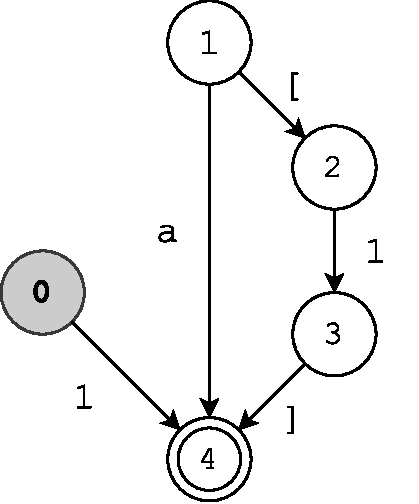
\includegraphics[width=4cm]{Kovalev/pictures/ra_example.pdf}
		\caption{Рекурсивный автомат для $G_1$}
	\caption{КС-грамматика и эквивалентный ей рекурсивный автомат}
	\label{fig:ra_ex}
\end{figure}

\subsection{GLL-алгоритм и его модификации}

Классические алгоритмы нисходящего и восходящего синтаксического анализа предполагают использование грамматики, которая является в достаточной мере однозначной. 
В противном случае, управляющие таблицы анализаторов содержат конфликты, из-за чего нельзя гарантировать корректное поведение на любых входных данных. 
Для работы с сильно неоднозначными грамматиками используются алгоритмы \textit{обобщенного синтаксического анализа}, которые позволяют рассмотреть все возможные пути разбора строки и построить соответствующие деревья вывода.
Поиск шаблонов не требует наличия деревьев вывода, поэтому в дальнейшем алгоритмы синтаксического анализа рассматриваются только как механизм, позволяющий определить принадлежность строки языку.

\subsubsection{Оригинальный GLL-алгоритм}

Generalized LL (GLL) --- алгоритм, обобщающий идеи нисходящего синтаксического анализа. GLL, в отличие от стандартных алгоритмов LL-класса, позволяет использовать для анализа произвольную \linebreak контекстно-свободную грамматику, в том числе содержащую леворекурсивные правила. Вместе с тем, GLL наследует такие полезные свойства алгоритмов нисходящего анализа, как непосредственная связь с грамматикой и простота отладки и диагностики ошибок.

Для обработки неоднозначностей GLL разделяет стек анализатора на несколько ветвей, каждая из которых соответствует возможному пути разбора. При таком подходе необходимо компактное представление множества стеков, в качестве которого выступает Graph Structured Stack (GSS). В работе \cite{Afroozeh2015gss} была представлена модификация GSS, которая позволяет увеличить эффективность GLL-анализа. Вершины такого представления хранят в себе номер нетерминала и позицию в строке, с которой начался разбор подстроки, соответствующей ему. На ребрах хранятся позиции в грамматике (вида $X \rightarrow \alpha A \cdot \beta$), на которые необходимо вернуться после завершения разбора нетерминала. 
%При помощи GSS также решается проблема бесконечного роста стеков при обработке левой рекурсии: при попытке создать вершину, которая уже существует, в граф добавится

Основной идеей GLL является использование \textit{дескрипторов}, позволяющих полностью описывать состояние анализатора в текущий момент времени.

\begin{defn}
	Дескриптор --- это тройка (L, u, i), где:
	\begin{itemize}
		\setlength\itemsep{0em}
		\item L --- текущая позиция в грамматике вида $A \rightarrow \alpha \cdot \beta$;
		\item u --- текущая вершина GSS;
		\item i --- позиция во входном потоке.
	\end{itemize}
\end{defn}  

В процессе работы поддерживается глобальная очередь дескрипторов. В начале каждого шага исполнения алгоритм берет следующий в очереди дескриптор и производит действия в зависимости от позиции в грамматике и текущего входного символа, передвигая соответствующие указатели. 
При наличии конфликтов в грамматике алгоритм добавляет дескрипторы для каждого возможного пути анализа в конец очереди.

\subsubsection{Поддержка грамматик в EBNF}

В работе \cite{Gorokhov2017ebnf} была описана модификация GLL, которая позволяет использовать грамматики, записанные в расширенной форме Бэкуса-Наура (EBNF). Грамматика такого вида трансформируется в соответствующий рекурсивный автомат, в котором затем минимизируется количество состояний. Синтаксический анализ производится без построения управляющих таблиц: алгоритм обходит рекурсивный автомат в соответствии со входным потоком символов. При обработке текущего дескриптора $(C_S, C_U, i)$, где $C_S$ --- вершина автомата (эквивалент позиции в грамматике), $C_U$ --- вершина GSS, $i$ --- позиция в строке, могут возникать следующие ситуации.

\begin{itemize}
	\item $C_S$ --- финальное состояние. Показывает, что разбор текущего нетерминала завершен. Необходимо осуществить возврат из $C_U$ по меткам на исходящих из нее ребрах.
	\item Присутствует нетерминальный переход из $C_S$. В данном случае необходимо начать разбор указанного нетерминала $X$. Для этого в GSS должна быть создана новая вершина $(X, i)$, если таковой не было ранее, а текущая вершина автомата изменена на стартовую для $X$.
	\item Присутствует терминальный переход из $C_S$. Необходимо сравнить терминал на ребре автомата с текущим входным символом. Если они совпадают, то осуществить переход в вершину автомата, на которую указывает ребро, и передвинуть указатель в строке.
\end{itemize}

За счет уменьшения количества состояний в автомате удается достичь прироста в производительности по сравнению со стандартным GLL-алгоритмом.

\subsubsection{Синтаксический анализ графов}

Стандартными входными данными для алгоритмов синтаксического анализа являются линейные последовательности токенов. На основе GLL был разработан алгоритм, который позволяет производить синтаксический анализ регулярных множеств строк, представленных в виде конечного автомата (который, в свою очередь, является ориентированным графом с токенами на ребрах).

Поддержка нелинейного входа не потребовала существенных изменений в оригинальном алгоритме. Дескрипторы модифицированного алгоритма хранят номер вершины входного графа вместо позиции в строке. Также, на шаге исполнения просматривается не единственный текущий символ, а множество символов на ребрах, исходящих из текущей вершины.

Производительность данного алгоритма, как и обычного GLL, может быть увеличена при помощи представления входной грамматики в виде рекурсивного автомата. В таком случае, алгоритм будет производить обход двух автоматов --- рекурсивного и конечного. Ситуации, возникающие при обработке дескрипторов, не отличаются от описанных ранее ситуаций для линейного входа. Псевдокод данной модификации приведен в приложении. Рассматривается вариант без построения деревьев вывода, алгоритм возвращает длины корректных цепочек, порождаемых автоматом. 

\subsection{Проект YaccConstructor}

YaccConstructor \cite{SemyonPhD} --- исследовательский проект лаборатории языковых инструментов JetBrains на математико-механическом факультете СПбГУ, направленный на исследования в области лексического и синтаксического анализа. Проект включает в себя одноименную модульную платформу для разработки лексических и синтаксических анализаторов, содержащую большое количество компонент: язык описания грамматик YARD \cite{yard_url}, преобразования над грамматиками и др. Основным языком разработки является F$\#$.

Ранее в рамках YaccConstructor были реализованы генераторы GLL-анализаторов, описание которых было приведено в данном обзоре. 
